\section{Objectives}
Follow Lab 12 (PDF pages 52--54) to compare size-dependent delay in five-stage chains and evaluate taper factors for five stages driving 2 pF.

\section{Specification mapping}
\begin{longtable}{p{0.31\linewidth}p{0.29\linewidth}p{0.31\linewidth}}
\toprule
Handout requirement (PDF page) & Implementation & Verification and scope \\\midrule
Step 1: all four Table 12.1 sizes (52,54) & 01\_delay\_elements & Four parallel five-stage chains \\
Step 2: change taper n (53--54) & 02\_taper\_buffer & Five stages, n=2/3/4/5, $C_L=2$ pF \\
\bottomrule
\end{longtable}


\section{Circuit and design derivation}
The first part uses all four numerical $W_p,W_n,L$ entries in Table 12.1. Case 2 lists $W_p=1.2\,\mu$m, while the prose calls it half of case 1 (which would be 1.8). This implementation follows the table and records the inconsistency. The altered dimensions and ratios in the reference code are restored to the table. For the taper, stage k widths equal the first-stage widths times $n^{k-1}$. Length is fixed at $0.25\,\mu$m and first-stage $W_n/W_p=0.6/1.8\,\mu$m. The final 2 pF load corrects the reference code's 1 pF.

The estimate $t\sim RC$ explains the tradeoff: wider devices reduce channel resistance but add self and downstream capacitance, so total delay need not decrease monotonically.

\section{Simulation setup}
This teaching rewrite uses a separately supplied model at 1.0 V and $25\,^{\circ}\mathrm C$. The specified topology, loads and comparative dimensions are retained. The handout's 2.5 V process results are not acceptance values for this model. The chosen 1 V is a simulation condition, not a verified device rating. MOS bulk terminals are explicitly connected to the corresponding supply rails.

HSPICE S-2021.09 uses RUNLVL=6, retaining waveforms, printed data and native measurements. Figures are redrawn from actual data; CSV files are in each Lab's results directory. Successful solution does not establish process reliability. Warnings from encrypted model blocks remain suppressed; the existing diagnostic did not expose actionable further details, so the warnings are not declared harmless and complete model-limit compliance is not claimed.

Delay chains use 0.1 ns input edges, a 5 ns period and 15 ns simulation. The taper uses the same edge rate, a 2 ns initial delay, 20 ns high interval, 45 ns period and 90 ns duration to allow settling of the large load. Delays run from the input 50\% crossing to the opposite-polarity stage-5 50\% crossing; both $t_{pHL}$ and $t_{pLH}$ are reported.

\section{Results and specification checks}
All five parameter cases completed normally. Dimensions are in $\mu$m and delays in ns.
\begin{center}\small
\begin{tabular}{llllll}
\toprule
Case & $W_p$ & $W_n$ & $L$ & $t_{pHL}$ & $t_{pLH}$ \\
\midrule
1 & 3.6 & 1.2 & 0.25 & 0.3634 & 0.3786 \\
2 & 1.2 & 1.2 & 0.25 & 0.3515 & 0.3926 \\
3 & 3.6 & 1.2 & 0.5 & 1.2781 & 1.3400 \\
4 & 1.8 & 1.2 & 0.5 & 1.2200 & 1.3434 \\
\bottomrule
\end{tabular}
\end{center}

\begin{figure}[htbp]
\centering
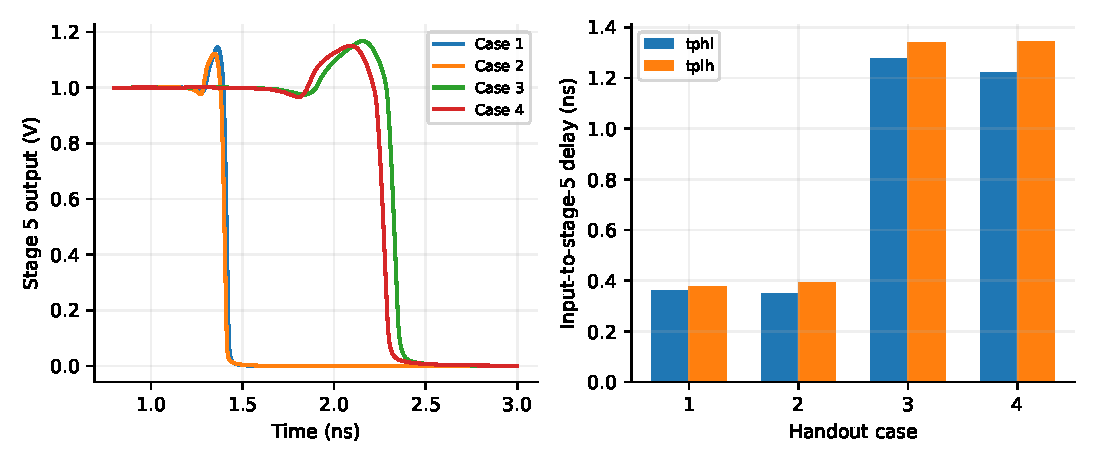
\includegraphics[width=\linewidth]{figures/delay_elements.pdf}
\caption{Results for the four delay-element sizes; redrawn from this run's HSPICE data.}
\end{figure}
\begin{center}\small
\begin{tabular}{llll}
\toprule
n & $t_{pHL}$ (ns) & $t_{pLH}$ (ns) & Mean (ns) \\
\midrule
2 & 0.9314 & 1.1852 & 1.0583 \\
3 & 0.8779 & 0.9877 & 0.9328 \\
4 & 0.9924 & 1.3381 & 1.1652 \\
5 & 1.5245 & 2.2524 & 1.8884 \\
\bottomrule
\end{tabular}
\end{center}

\begin{figure}[htbp]
\centering
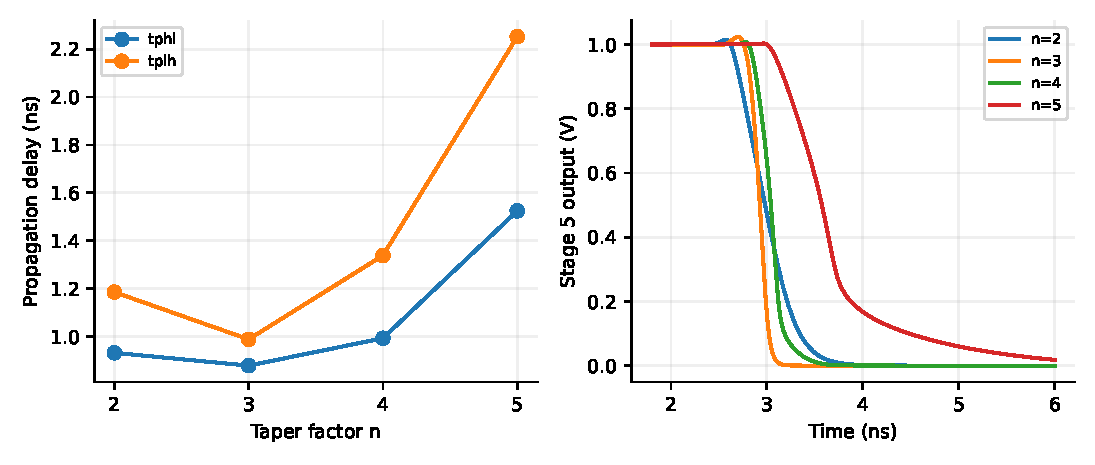
\includegraphics[width=\linewidth]{figures/taper_buffer.pdf}
\caption{Taper comparison at five stages and 2 pF; redrawn from this run's HSPICE data.}
\end{figure}


\section{Discussion}
Longer channels substantially increase delay, while reduced PMOS width affects the two transition directions differently. Cases 1 and 2 have nearly equal mean delays in this model, so the handout's single-delay ordering is not universal. Among n=2--5, n=3 gives the smallest mean delay, about 0.933 ns. This matches the handout's best-factor trend, not its 0.449 ns value. Other stage counts, non-geometric sizes and loads were not searched, so global optimality is not claimed.

\section{Conclusion}
Both steps are covered with explicit resolution of the table/prose conflict, the specified 2 pF load and five-stage topology. Conclusions are limited to the tested parameter set.
